\documentclass[aspectratio=169,handout]{beamer}

\usepackage[utf8]{inputenc}
\usepackage{lmodern}
\usepackage{pgfplots} \pgfplotsset{compat=1.13} % also includes tikz
\usepgfplotslibrary{fillbetween}
\usetikzlibrary{external} % To speed up compile
\tikzexternalize
% \usepackage{svg} % automatically convert svg and include

\usetheme{Goettingen} % To show sidebar navigation
\setbeamercolor{paleBlue}{fg=black,bg=blue!10!white}

\colorlet{paleBlue}{blue!10!white}
\colorlet{halfBlue}{blue!50!white}
 
%%%%%%%%% helpers
\newcommand{\abs}[1]{\left|#1\right|} % Absolute value
\newcommand{\norm}[1]{\left\|#1\right\|} % Norm
\newcommand{\bC}{\mathbb{C}} % Complex numbers
\newcommand{\bN}{\mathbb{N}} % Natural numbers
\newcommand{\bR}{\mathbb{R}} % Real numbers
\renewcommand{\aa}{\mathbf{a}}
\newcommand{\bb}{\mathbf{b}}
\newcommand{\cc}{\mathbf{c}}
\newcommand{\ee}{\mathbf{e}}
\newcommand{\ff}{\mathbf{f}}
\renewcommand{\gg}{\mathbf{g}}
\newcommand{\hh}{\mathbf{h}}
\newcommand{\rr}{\mathbf{r}}
\newcommand{\uu}{\mathbf{u}}
\newcommand{\vv}{\mathbf{v}}
\newcommand{\ww}{\mathbf{w}}
\newcommand{\xx}{\mathbf{x}}
\newcommand{\yy}{\mathbf{y}}
\newcommand{\zz}{\mathbf{z}}
\newcommand{\aalpha}{\boldsymbol{\alpha}}
\newcommand{\bbeta}{\boldsymbol{\beta}}
\newenvironment{shaded}{\begin{beamercolorbox}[sep=.1em,rounded=true]{paleBlue}}{\end{beamercolorbox}}



%%%%%%%%%

\title{MA2 -- Part 5 -- Multiple integrals}
\subtitle{Weeks 9--10 of MA2 -- Draft lecture slides}
\author[]{Oliver Butterley}
\institute{University of Rome Tor Vergata}
\date{2020/21}
\setbeamercovered{transparent} 

\begin{document}

\frame{\titlepage}

\begin{frame}
    \frametitle{Outline}
    \tableofcontents
\end{frame}

\section{Definition of integrability and properties of the integral}

\begin{frame}
    \frametitle{Plan of action}
    \structure{Recall:}
    One-dimensional case
    \begin{enumerate}
        \item define the integral for step functions;
        \item define integral for ``integrable functions'';
        \item  show that continuous functions are integrable.
    \end{enumerate}

    For higher dimensions we follow the same logic. We will then show that we can evaluate higher dimensional integrals by repeated one-dimensional integration.



\end{frame}


\subsection{Partitions of rectangles and step functions}

\begin{frame}
    \frametitle{Partitions of rectangles}


    \begin{columns}
        \begin{column}{.5\textwidth}

            \structure{Observe:}

            \begin{itemize}
                \item             Partition divides \(R\) into \(nm\) sub-rectangles.
                \item If \(P \subseteq Q\) then we say that \(Q\) is a finer partition than \(P\).

            \end{itemize}
        \end{column}
        \begin{column}{.5\textwidth}

            \begin{figure}
                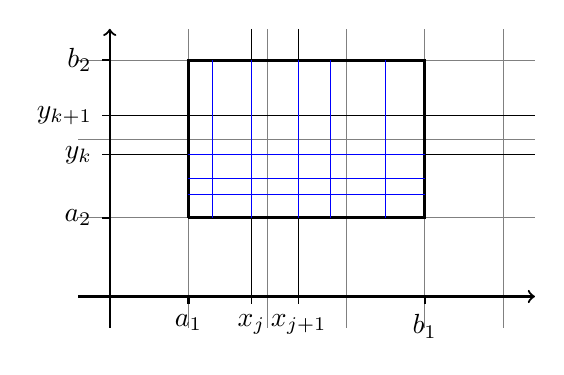
\begin{tikzpicture}
                    \draw[step=1cm,gray,very thin] (-0.4,-0.4) grid (5.4,3.4);
                    \draw[thick,->] (-0.4,0) -- (5.4,0);
                    \draw[thick,->] (0,-0.4) -- (0,3.4);
                    \draw[very thick] (1,1) -- (4,1) -- (4,3) -- (1,3) -- (1,1);
                    \draw[thick] (1,0) -- (1,-.1) node[below] {\(a_1\)};
                    \draw[thick] (4,0) -- (4,-.1) node[below] {\(b_1\)};
                    \draw[thick] (0,1) -- (-.1,1) node[left] {\(a_2\)};
                    \draw[thick] (0,3) -- (-.1,3) node[left] {\(b_2\)};
                    \draw[] (5.4,1.8) -- (-.1,1.8) node[left] {\(y_{k}\)};
                    \draw[] (5.4,2.3) -- (-.1,2.3) node[left] {\(y_{k+1}\)};
                    \draw[blue]
                    (1,1.3) -- (4,1.3)
                    (1,1.5) -- (4,1.5)
                    (1,1.8) -- (4,1.8);
                    (1,2.3) -- (4,2.3)
                    \draw[] (1.8,3.4) -- (1.8,-.1) node[below] {\(x_j\)};
                    \draw[] (2.4,3.4) -- (2.4,-.1) node[below] {\(x_{j+1}\)};
                    \draw[blue]
                    (1.3,1) -- (1.3,3)
                    (1.8,1) -- (1.8,3)
                    (2.4,1) -- (2.4,3)
                    (2.8,1) -- (2.8,3)
                    (3.5,1) -- (3.5,3);
                \end{tikzpicture}
                \caption{A partition of a rectangle \(R\).}
            \end{figure}


        \end{column}
    \end{columns}


    \begin{definition}[partition]
        Let \(R = [a_1,b_1] \times [a_2,b_2]\) be a rectangle.
        Suppose that \(P_1 = \{x_0,\ldots,x_m\}\) and \(P_2 = \{y_0,\ldots,y_n\}\) such that
        \(a_1 = x_0 < x_2 < \cdots < x_m = b_1\) and \(a_2 = y_0 < y_2 < \cdots < y_n = b_2\).
        \(P= P_1 \times P_2\) is said to be a partition of \(R\).
    \end{definition}



\end{frame}


\begin{frame}
    \frametitle{Step functions}

    \begin{definition}[step function]
        A function \(f:R\to \bR \) is said to be a \emph{step function} if there is a partition \(P\) of \(R\) such that \(f\) is constant on each sub-rectangle of the partition.
    \end{definition}



    \begin{columns}
        \begin{column}{.5\textwidth}
            \begin{figure}
                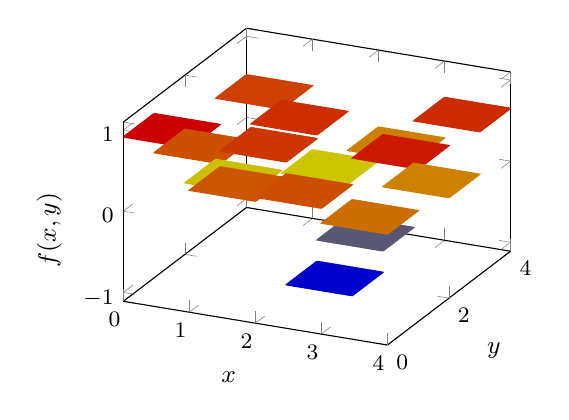
\begin{tikzpicture}
                    \begin{axis}[
                            xlabel={$x$}, ylabel={$y$}, zlabel={$f(x,y)$},
                            xmin = 0, xmax = 4, ymin = 0, ymax = 4,
                            small,
                        ]
                        \foreach \xindex in {1,2,3,4}
                        \foreach \yindex in {1,2,3,4}
                        \pgfmathsetmacro{\xi}{rand}
                        \addplot3[
                            surf,
                            domain={\xindex-1}:\xindex,
                            domain y={\yindex-1}:\yindex,
                        ]
                        {\xi};
                    \end{axis}
                \end{tikzpicture}
                \caption{Graph of a step function.}
            \end{figure}
        \end{column}
        \begin{column}{.5\textwidth}
            \begin{itemize}
                \item If \(f\) and \(q\) are step functions and  \(c,d \in \bR\), then \(c f + d g\) is also a step function;
                \item The area of the sub-rectangle \(Q_{jk}:=[x_{j},x_{j+1}]\times [y_{k},y_{k+1}]\) is equal to \( (x_{j+1}-x_{j})(y_{k+1}-y_{k})\).
            \end{itemize}

        \end{column}
    \end{columns}

\end{frame}

\subsection{Integral of a step function}

\begin{frame}
    \frametitle{Integral of a step function}

    \begin{definition}[integral of a step function]
        Suppose that \(f\) is a step function with value \(c_{jk}\) on the sub-rectangle \((x_{j},x_{j+1})\times (y_{k},y_{k+1})\).
        Then we define the integral as
        \[
            \iint_{R} f \ dxdy = \sum_{j=0}^{m-1} \sum_{k=0}^{n-1} c_{jk} (x_{j+1}-x_{j})(y_{k+1}-y_{k}).
        \]
    \end{definition}

    \begin{itemize}
        \item The value of the integral is independent of the partition, as long as the function is constant on each sub-rectangle,
        \item If \(Q_{jk} = (x_{j},x_{j+1})\times (y_{k},y_{k+1})\) then
              \[
                  \begin{aligned}
                      \iint_{Q_{jk}} f \ dxdy & = c_{jk} (x_{j+1}-x_{j})(y_{k+1}-y_{k})                                       \\
                                              & = \int_{x_j}^{x_{j+1}} \left[\int_{y_k}^{y_{k+1}}f(x,y) \ dy\right] \ dx
                                              & =  \int_{y_k}^{y_{k+1}} \left[ \int_{x_j}^{x_{j+1}} f(x,y) \ dx \right] \ dy.
                  \end{aligned}
              \]
    \end{itemize}

\end{frame}

\begin{frame}
    \frametitle{Properties of the integral of step functions}

    \begin{theorem}[basic properties of the integral]
        Let \(f,g\) be step functions.
        \begin{enumerate}
            \item \(\displaystyle \iint_{R} (a f + b g) \ dxdy = a \displaystyle \iint_{R} f \ dxdy + b \displaystyle\iint_{R} g \ dxdy\) for all \(a,b\in \bR\);
            \item \(\displaystyle\iint_{R} f \ dxdy =  \displaystyle\iint_{R_1} f \ dxdy + \displaystyle \iint_{R_2} f \ dxdy\) if \(R\) is divided into \(R_1\) and \(R_2\);
            \item \(\displaystyle\iint_{R} f \ dxdy \leq \displaystyle \iint_{R} g \ dxdy\) if \(f(x,y) \leq g(x,y)\).
        \end{enumerate}
    \end{theorem}

    \begin{proof}
        Straightforward from the definition.
    \end{proof}


\end{frame}

% \begin{frame}
%     \frametitle{Upper and lower integrals}

%     \begin{definition}[integrability]
%         Let \(R\) be a rectangle and let \(f: R \to \bR\) be a bounded function.
%         \begin{itemize}
%             \item The lower integral \(\underline{I}\) is defined to be the supremum of \(\iint_{R} \underline{g} \ dxdy\) where \(\underline{g}\) is any step function such that \(\underline{g} \leq f\).
%             \item The upper integral \(\overline{I}\) is defined to be the infimum of \(\iint_{R} \overline{g} \ dxdy\) where \(\underline{g}\) is any step function such that \(f \leq \overline{g}\).
%             \item \(f\) is said to be \emph{integrable} if \(\underline{I}=\overline{I}\). In this case we say that  
%             \[\iint_{R} f \ dxdy = \underline{I}=\overline{I}.\]
%         \end{itemize}
%     \end{definition}

% \end{frame}

\subsection{Definition of integrable}


\begin{frame}
    \frametitle{Upper / lower integrals and integrability}

    \begin{definition}[integrability]
        Let \(R\) be a rectangle and let \(f: R \to \bR\) be a bounded function.
        If there is one and only one number \(I\in \bR\) such that
        \[
            \iint_{R} g(x,y) \ dxdy \leq I \leq \iint_{R} h(x,y) \ dxdy
        \]
        for every pair of step functions \( g, h\) such that, for all \((x,y)\in R\),
        \[
            g(x,y) \leq f(x,y) \leq h(x,y).
        \]
        This number \(I\) is called the integral of \(f\) on \(R\) and is denoted \(\iint_{R} f(x,y) \ dxdy\).
    \end{definition}


\end{frame}


\subsection{Evaluation of an integral}


\begin{frame}
    \frametitle{}

    \begin{theorem}[evaluating by repeated integration]
        Let \(f\) be a bounded integrable function on  \(R = [a_1,b_1] \times [a_2,b_2]\).
        Suppose that, for every \(y\in [a_2,b_2]\), the integral \(\int_{a_1}^{b_1} f(x,y) \ dx =: A(y)\) exists.
        Then \(\int_{a_2}^{b_2} A(y) \ dy\) exists and
        \vspace{-1em}
        \[
            \iint_{R} f \ dxdy = \int_{a_2}^{b_2} \left[ \int_{a_1}^{b_1} f(x,y) \ dx  \right] \ dy.
        \]
    \end{theorem}
    \vspace{-1em}
    \begin{proof}
        \begin{enumerate}
            \item Choose step functions \(g,h\) such that \(g\leq f \leq h\),
            \item By assumption \(\int_{a_1}^{b_1} g(x,y) \ dx \leq A(y) \leq \int_{a_1}^{b_1} h(x,y) \ dx,  \)
            \item Observe that \(\int_{a_1}^{b_1} g(x,y) \ dx \) and \(\int_{a_1}^{b_1} h(x,y) \ dx\) are step functions (in \(y\)) and so \(A(y)\) is integrable and, moreover,
                  \[ \hspace{-2em}
                      \int_{a_2}^{b_2} \left[ \int_{a_1}^{b_1} g(x,y) \ dx  \right] \ dy
                      \leq \int_{a_2}^{b_2} \left[ \int_{a_1}^{b_1} f(x,y) \ dx  \right] \ dy
                      \leq \int_{a_2}^{b_2} \left[ \int_{a_1}^{b_1} h(x,y) \ dx  \right] \ dy.
                  \]
        \end{enumerate}
    \end{proof}

\end{frame}




\begin{frame}
    \frametitle{Integrability of continuous functions}

    \begin{theorem}[integral of continuous functions]
        Suppose that \(f\) is a continuous function defined on the rectangle \(R\).
        Then \(f\) is integrable and
        \[
            \iint_{R} f(x,y) \ dxdy
            = \int_{a_2}^{b_2} \left[ \int_{a_1}^{b_1} f(x,y) \ dx  \right] \ dy
            = \int_{a_1}^{b_1} \left[\int_{a_2}^{b_2}  f(x,y) \ dy  \right] \ dx.
        \]
    \end{theorem}
    \begin{proof}
        \begin{enumerate}
            \item Continuity implies boundedness and so upper and lower integrals exist,
            \item Let \(\epsilon>0\). Exists \(\delta>0\) such that \(\abs{f(\xx)-f(\yy)}\leq \epsilon\) whenever \(\norm{\xx-\yy}\leq \delta\),
            \item Partition such  \(\norm{\xx-\yy}\leq \delta\) whenever \(\xx,\yy\) are in the same sub-rectangle \(Q_{jk}\),
            \item Step functions \(g,h\) s.t. \(g(\xx)=\inf_{Q{jk}} f\),   \(h(\xx)=\sup_{Q{jk}} f\) when \(\xx\in Q_{jk}\),
            \item \(\abs{\inf_{Q{jk}} f - \sup_{Q{jk}} f }\leq \epsilon\) and \(\epsilon>0\) can be made arbitrarily small.
        \end{enumerate}
    \end{proof}

\end{frame}




\begin{frame}
    \frametitle{Volume of a solid}
    Let \(f(x,y)\) be positive on the rectangle \(R \subset \bR^2\) and consider the 3D set
    \[
        V := \left\{(x,y,z): (x,y)\in R, 0 \leq z \leq f(x,y)\right\}.
    \]

    \begin{columns}
        \begin{column}{.5\textwidth}
            \begin{figure}
                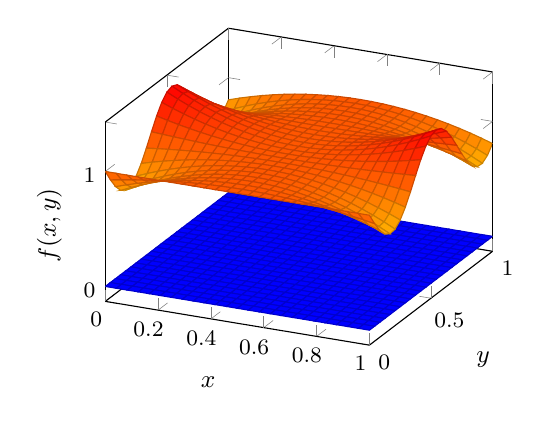
\begin{tikzpicture}
                    \begin{axis}[
                            xlabel={$x$}, ylabel={$y$}, zlabel={$f(x,y)$},
                            xmin = 0, xmax = 1, ymin = 0, ymax = 1,
                            small,
                        ]
                        \addplot3[
                            surf,
                            domain=0:1,
                            domain y=0:1,
                        ]{0};
                        \addplot3[
                            surf,
                            domain=0:1,
                            domain y=0:1,
                        ]{1 - 1.2* (x-.5)*(x-.5)*sin(500*y)};
                    \end{axis}
                \end{tikzpicture}
                \caption{Set enclosed by \(xy\)-plane \& \(f(x,y)\).}
            \end{figure}
        \end{column}
        \begin{column}{.5\textwidth}

            \begin{itemize}
                \item  The volume of the set is equal to
                      \[
                          \operatorname{Vol}(V) = \iint_{R} f(x,y) \ dxdy.
                      \]
                \item Also possible: \(f(x,y)\leq z \leq g(x,y)\).
            \end{itemize}
        \end{column}
    \end{columns}
\end{frame}


\begin{frame}
    \frametitle{Functions with discontinuities}

    \begin{definition}[content zero set]
        A bounded subset \(A\subset \bR^2\) is said to have content zero if, for every \(\epsilon>0\), there exists a finite set of rectangles whose union includes \(A\) and the sum of the areas of the rectangles is not greater than \(\epsilon\).
    \end{definition}



    \begin{columns}
        \begin{column}{.5\textwidth}


            \begin{example}
                \begin{itemize}
                    \item Finite set of points,
                    \item Bounded segment,
                    \item Continuous path.
                \end{itemize}
            \end{example}

        \end{column}
        \begin{column}{.5\textwidth}

            \begin{figure}
                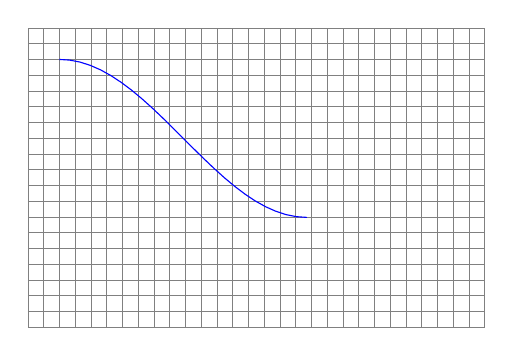
\begin{tikzpicture}
                    \draw[step=.2cm,gray,very thin] (-0.4,-0.4) grid (5.4,3.4);
                    \draw [blue, domain=0:pi] plot (\x, {2+cos(\x r)*exp(\x/exp(2*pi))});
                \end{tikzpicture}
                \caption{The graph of a continuous function has content zero.}
            \end{figure}

        \end{column}
    \end{columns}


\end{frame}


\begin{frame}
    \frametitle{Integrating functions with discontinuities}

    \begin{theorem}
        Let \(f\) be a bounded function on \(R\) and suppose that the set of discontinuities \(A\subset R\) had content zero. Then the double integral \(\iint_{R}f(x,y) \ dxdy\) exists.
    \end{theorem}
    \begin{proof}
        \begin{enumerate}
            \item Take a cover of \(A\) by rectangles with total area not greater than \(\delta>0\),
            \item Let \(P\) be a partition of \(R\) which is finer than the cover of \(A\),
            \item We may assume that \(\abs{\inf_{Q{jk}} f - \sup_{Q{jk}} f }\leq \epsilon\)  on each sub-rectangle of the partition which doesn't contain a discontinuity of \(f\),
            \item The contribution to the integral of bounding step functions from the cover of \(A\) is bounded by \(\delta \sup \abs{f}\).
        \end{enumerate}
    \end{proof}


\end{frame}



\begin{frame}
    \frametitle{Integrals over regions bounded by continuous functions}


    \begin{definition}[integral on general regions]
        Suppose \(S\subset R\) and \(f\) is a bounded function on \(S\).
        We extend \(f\) to \(R\) by defining
        \[
            f_R(x,y) := \begin{cases}
                f(x,y) & \text{if \((x,y)\in S\)} \\
                0      & \text{otherwise}.
            \end{cases}
        \]
        We say that \(f\) is integrable if \(f_{R}\) is integrable and define
        \[
            \iint_{S} f(x,y) \ dxdy = \iint_{R} f_{R}(x,y) \ dx dy.
        \]
    \end{definition}

\end{frame}

\begin{frame}
    \frametitle{Regions bounded by continuous functions}



    \begin{columns}
        \begin{column}{.54\textwidth}
            \begin{definition}[type 1]
                \(S \subset \bR^2\) is \emph{type 1} if there are continuous functions \(\varphi_1\), \(\varphi_2\) such that
                \[
                    S = \left\{(x,y): x \in [a,b], \varphi_1(x) \leq y \leq \varphi_2(x)\right\}.
                \]
            \end{definition}
            \begin{definition}[type 2]
                \(S \subset \bR^2\) is \emph{type 2} if there are continuous functions \(\varphi_1\), \(\varphi_2\) such that
                \[
                    S = \left\{(x,y): y \in [a,b], \varphi_1(y) \leq x \leq \varphi_2(y)\right\}.
                \]
            \end{definition}

        \end{column}
        \begin{column}{.46\textwidth}

            \begin{figure}
                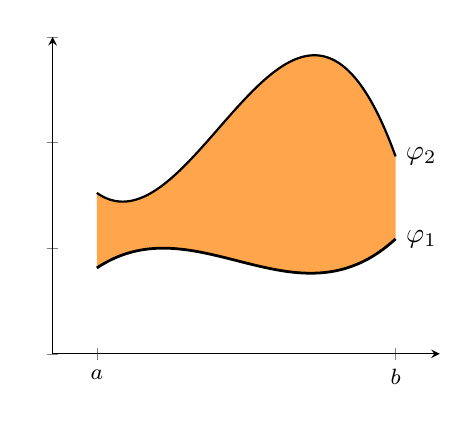
\begin{tikzpicture}
                    \begin{axis}[
                            axis y line = left,
                            axis x line = bottom,
                            xtick       = {-1.2,4.2},
                            xticklabels = {$a$,$b$},
                            yticklabels=\empty,
                            samples     = 160,
                            domain      = -1.2:4.2,
                            xmin = -2, xmax = 5,
                            ymin = -5, ymax = 10,
                            small,
                        ]
                        \addplot[name path=top, black, thick, mark=none, ] {-x^3/3 + (x^2) + 2*x + 3} node[right]{\(\varphi_2\)};
                        \addplot[name path=bottom, black, no markers, line width=1pt] {x^3/8-x^2/2} node[right]{\(\varphi_1\)};
                        \addplot fill between[
                                of = top and bottom,
                                every even segment/.style = {orange!70},
                            ];
                    \end{axis}
                \end{tikzpicture}
                \caption{A region of type 1.}
            \end{figure}

        \end{column}
    \end{columns}
\end{frame}


\begin{frame}
%    \frametitle{Integrals over regions bounded by continuous functions}

    \begin{theorem}
        Let \(\varphi\) be a continuous function on \([a,b]\). 
        Then the graph 
        \(\left\{(x,y): x\in [a,b], y=\varphi(x)\right\}\)
        has zero content.
    \end{theorem}
    \begin{proof}
        \begin{enumerate}
            \item Continuity means that, for every \(\epsilon>0\), there exists \(\delta>0\) such that \(\abs{\varphi(x) - \varphi(y)}\leq \epsilon\) whenever \(\abs{x-y}\leq \delta\),
            \item Take partition of \([a,b]\) into subintervals of length less than \(\delta\),
            \item Using this partition we generate a cover of the graph which has area not greater than \(2\epsilon \abs{b-a}\).
        \end{enumerate}
    \end{proof}

\end{frame}

\begin{frame}
    \frametitle{Integrals over regions bounded by continuous functions}
    

    \begin{theorem}
        Let \(S = \left\{(x,y): x \in [a,b], \varphi_1(x) \leq y \leq \varphi_2(x)\right\}\) be a region of type 1 and let \(f\) be a bounded continuous function of \(S\).
        Then \(f\) is integrable on \(S\) and
        \[
            \iint_{S} f(x,y) \ dxdy = \int_{a}^{b} \left[\int_{\varphi_1(x)}^{\varphi_2(x)} f(x,y) \ dy\right] \ dx.
        \] 
    \end{theorem}
    
    \begin{proof}
        \begin{enumerate}
            \item The set of discontinuity of \(f_{R}\) is the boundary of \(S\) in \(R=[a,b]\times[\tilde a,\tilde b]\) which consists of the graphs of \(\varphi_1\), \(\varphi_2\),
            \item These graphs have zero content as we proved before,
            \item For each \(x\), \(f(x,y)\) is integrable since it has only two discontinuity points,
            \item Additionally \(\int_{\tilde a}^{\tilde b} f_{R}(x,y) \ dy =  \int_{\varphi_1(x)}^{\varphi_2(x)} f(x,y) \ dy \). \qedhere
        \end{enumerate}
    \end{proof}

    \structure<>{Remark:} A similar result holds for type 2 regions.
\end{frame}

\subsection{Applications of multiple integrals}

\begin{frame}
    % \frametitle{Area and Volume}
 
        \begin{block}<>{Area of \(S\)}<>
            Let    \(S \subset \bR^2\)  be a \emph{type 1} region, i.e.,   \(\varphi_1\), \(\varphi_2\) are continuous functions,
            \[ 
                S := \left\{(x,y): x \in [a,b], \varphi_1(x) \leq y \leq \varphi_2(x)\right\}.
            \]
            Integrating:
            \[
                \iint_{S} \ dx dy = \int_{a}^{b}( \varphi_2(x) - \varphi_1(x)) \ dx.
            \]
        \end{block}

        \begin{block}<>{Volume of \(V\)}<>
            Let \(f(x,y) \geq g(x,y)\) be continuous functions on \(S\) and
            \[
                V := \left\{ (x,y,z) :  x \in [a,b], \varphi_1(x) \leq y \leq \varphi_2(x), f(x,y) \leq z \leq g(x,y)  \right\}.
            \]
            Integrating:
            \[
                \iiint_{V} \ dxdydz =  \int_{a}^{b}  
                \left[ \int_{\varphi_1(x)}^{\varphi_2(x)}   ( f(x,y)  -  g(x,y)) dy \right] \ dx.
            \]
        \end{block}
\end{frame}

\begin{frame}
    \frametitle{Mass, centre of mass, centroid}


    \begin{itemize}
        \item Suppose we have several particles\footnote{In general, mass \(m_k\) at point \(\xx_k\), the centre of mass is point \(\mathbf{X}\) such that \( M\mathbf{X} = \sum_{k} m_k \xx_k\).} each with mass \(m_k\) at point \((x_k,y_k)\).
            \begin{itemize}
                \item Total mass is \(M := \sum_{k} m_k\),
                \item Centre of mass is the point \((p,q)\) such that 
                \[ 
                    p M = \sum_{k} m_k x_k,
                    \quad 
                    q M = \sum_{k} m_k y_k.
                \] 
            \end{itemize}        
        \item Suppose a disk has the shape of a region \(S\) and the density of the material is \(f(x,y)\) at point \((x,y)\).
        \begin{itemize}
            \item Total mass is \(M := \iint_{S} f(x,y) \ dxdy\),
            \item Centre of mass is the point \((p,q)\) such that
            \[
                p M = \iint_{S} x \ f(x,y) \ dxdy, 
                \quad
                q M = \iint_{S} y \ f(x,y) \ dxdy.
            \] 
        \end{itemize}
        \item If the density is constant the centre of mass is called the centroid.
    \end{itemize}


\end{frame}

\section{Green's theorem}

\begin{frame}
    \frametitle{Green's theorem}

    \begin{theorem}[Green's theorem]
        Let \(C\subset\bR^2\) be a piecewise-smooth simple (no intersections) curve and \(\aalpha\) a path that parametrizes \(C\) in the counter-clockwise direction. 
        Let \(S\) be the region enclosed by \(C\).
        Suppose that \(\ff(x,y) = \left(\begin{smallmatrix}
            P(x,y) \\ Q(x,y)
        \end{smallmatrix}\right)\) is a vector field continuously differentiable  on an open set containing \(S\).
        Then
        \[
            \iint_{S} \left(\tfrac{\partial Q}{\partial x} - \tfrac{\partial P}{\partial y}\right) \ dxdy = \int_{C} \ff \cdot d\aalpha.
        \]
    \end{theorem}


\end{frame}

\begin{frame}
    \frametitle{}


    \begin{proof}[Proof of Green's theorem]
        \begin{enumerate}
            \item Assume that \(S\) is a type 1 region and that \(Q=0\),
            \item Since \(S = \left\{(x,y): x \in [a,b], \varphi_1(x) \leq y \leq \varphi_2(x)\right\}\),
            \[
                \iint_{S}  \left(\tfrac{\partial Q}{\partial x} - \tfrac{\partial P}{\partial y}\right) \ dxdy = 
                \int_{a}^{b}\left[\int_{\varphi_1(x)}^{\varphi_2(x)}  (- \tfrac{\partial P}{\partial y}) \ dy\right] \ dx
                = \int_{a}^{b}  (P(x,\varphi_1(x))-P(x,\varphi_2(x)))   dx,
            \]
            \item Choose paths \(\aalpha_1(t) = (t,\varphi_1(t))\), \(\aalpha_2(t) = (a,t)\), \(\aalpha_3(t) = (t,\varphi_2(t))\), \(\aalpha_4(t) = (b,t)\),
            \item \(\int_{C} \ff \cdot d\aalpha = \int \ff \cdot d\aalpha_1 - \int \ff \cdot d\aalpha_3 = \int_{a}^{b} P(t,\varphi_1(t)) \ dt -  \int_{a}^{b} P(t,\varphi_2(t)) \ dt \),
            \item If \(S\) is also type 2 then this works for \(P=0\) and linearity means it works for \(\ff = \left(\begin{smallmatrix}
                P \\ 0
            \end{smallmatrix}\right)+\left(\begin{smallmatrix}
                0 \\ Q
            \end{smallmatrix}\right)\),
            \item More general regions can be formed by ``glueing'' together simpler regions.
        \end{enumerate}
    \end{proof}
    

\end{frame}

\subsection{Simply connected regions}

\begin{frame}
    \frametitle{Simply connected regions}


    \begin{definition}[simply connected]
        The set \(S\subset \bR^n\) is said to be \emph{simply connected} if every closed path \(\aalpha(t)\) can be continuously shrunk to a point.
    \end{definition}
    \begin{columns}
        \begin{column}{.5\textwidth}

            \begin{figure}
                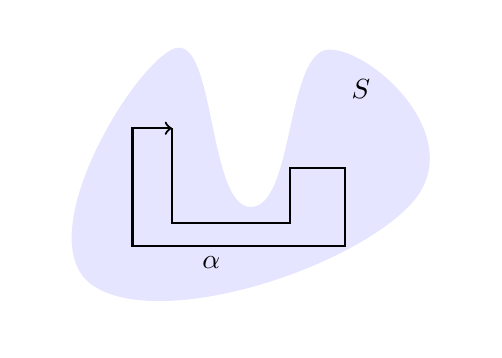
\begin{tikzpicture}
                    \fill[paleBlue] plot [smooth cycle, tension=1] coordinates {(0,0) (1,3) (2,1) (3,3) (4,1)};
                    \draw[->,thick] (1,2) -- (1,.8) -- (2.5,.8) -- (2.5,1.5) -- (3.2,1.5) -- (3.2,.5) -- (.5,.5) -- (.5,2) -- (1,2);
                    \node at (3.4,2.5){\(S\)};
                    \node at (1.5,0.3){\(\aalpha\)};
                \end{tikzpicture}
                \caption{Simply connected.}
            \end{figure}
        \end{column}

        \begin{column}{.5\textwidth}
            \begin{figure}
                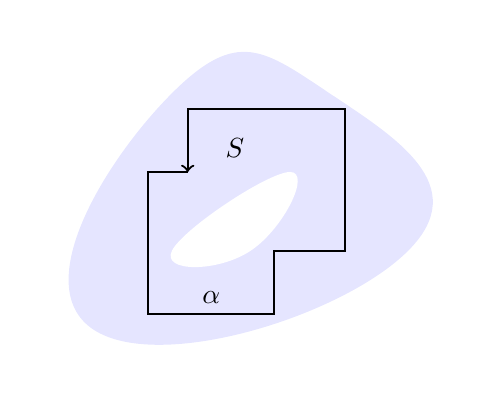
\begin{tikzpicture}
                    \fill[paleBlue] plot [smooth cycle, tension=1] coordinates {(0,0) (1,3) (3,3) (4,1)};
                    \fill[white] plot [smooth cycle, tension=1] coordinates {(1,1) (2,1) (2.5,2)};
                    \draw[->,thick] (1.2,2) -- (.7,2) -- (.7,.2) -- (2.3,.2) -- (2.3,1) -- (3.2,1) -- (3.2,2.8) -- (1.2,2.8) -- (1.2,2);
                    \node at (1.5,0.4){\(\aalpha\)};
                    \node at (1.8,2.3){\(S\)};
                \end{tikzpicture}
                \caption{Not simply connected.}
            \end{figure}
        \end{column}
    \end{columns}


\end{frame}





\subsection{Application to conservative vector fields}

\begin{frame}
    \frametitle{}


    \begin{theorem}[conservative vector fields on simply connected regions]
        Let \(S\) be a simply connected region and suppose that \(\ff = \left(\begin{smallmatrix}
            P \\ Q
        \end{smallmatrix}\right)\)
        is a vector field, continuously differentiable on \(S\).
        Then \(\ff\) is conservative if and only if \(\tfrac{\partial Q}{\partial x} = \tfrac{\partial P}{\partial y}\).
    \end{theorem}

    \begin{proof}
    \begin{enumerate}
        \item We already proved that \(\tfrac{\partial Q}{\partial x} = \tfrac{\partial P}{\partial y}\) whenever \(\ff\) is conservative;
        \item Now suppose that  \(\tfrac{\partial Q}{\partial x} = \tfrac{\partial P}{\partial y}\) and consider any closed path \(\aalpha\) in \(S\),
        \item By Green's theorem \(\int_{C} \ff \cdot d\aalpha = \iint_{S} \left(\tfrac{\partial Q}{\partial x} - \tfrac{\partial P}{\partial y}\right) \ dxdy = 0\),
        \item By the conservative vector field theorem this implies that \(\ff\) is conservative.
    \end{enumerate}    
    \end{proof}

    \structure{Remarks:} 
    \begin{itemize}
        \item     Invariance of a line integral under deformation of a path.
        \item Multiply connected regions.
    \end{itemize}
\end{frame}



\section{Change of variables}

\subsection{Jacobian determinant}

\begin{frame}
    \frametitle{Jacobian determinant}

    \structure<>{Recall 1D case:}
    If \(g : [a,b] \to [g(a),g(b)]\) is onto with continuous derivative and \(f\) is continuous then
    \[
      \int_{g(a)}^{g(b)}    f(x) \ dx = \int_{a}^{b} f(g(u)) \ g'(u) \ du.
    \]

    \begin{block}<>{Two dimensional change of coordinates}<>
        We consider maps \((u,v) \mapsto (X(u,v),Y(u,v))\) mapping  \(T\subset \bR^2\) to  \(S\subset \bR^2\).
        % \begin{itemize}
        %     \item Is the map differentiable?
        %     \item Is the map one-to-one?
        % \end{itemize}
        
    \end{block}

\end{frame}


\subsection{Change of variables}

\begin{frame}
    \frametitle{Change of variables}

    \begin{block}{Change of variables formula}
        Suppose that \((u,v) \mapsto (X(u,v),Y(u,v))\) which maps \(T\) to \(S\) is one-to-one with \(X\), \(Y\) continuously differentiable. Then
        \[
            \iint_{S} f(x,y) \ dxdy = \iint_{T} f(X(u,v),Y(u,v)) \ \abs{J(u,v)} \ dudv.
        \]
        where 
        \(J(u,v):= \begin{pmatrix}
            \partial_u X & \partial_u Y \\ \partial_v X & \partial_v Y
        \end{pmatrix}\) is the Jacobian matrix.
    \end{block}

    \begin{block}{Remark}
        The Jacobian is scaling of area: \(\displaystyle\iint_{S} \ dx dy = \displaystyle\iint_{T}  \abs{J(u,v)} \ dudv \).
    \end{block} 

\end{frame}

\subsection{Polar coordinates}

\begin{frame}
    \frametitle{Polar coordinates}

    Coordinate mapping:
    \begin{itemize}
        \item  \(x = r \cos \theta\)
        \item  \(y = r \sin \theta\)
    \end{itemize}

    Jacobian determinant:
    \[
        \abs{J(r,\theta)}
        = 
        \abs{\begin{pmatrix}
        \partial_u X & \partial_u Y \\ \partial_v X & \partial_v Y
        \end{pmatrix}}
        = 
        \abs{\begin{pmatrix}
        \cos \theta & \sin \theta \\ -r\sin \theta & r\cos \theta
        \end{pmatrix}}
        = r ( \cos^2\theta + \sin^2 \theta) = r.
    \]

    Change of coordinates:
    \[
        \iint_{S} f(x,y) \ dxdy = \iint_{T}  r  \ f(r\cos \theta, r\sin \theta)  \ drd\theta.
    \]

\end{frame}


\begin{frame}
    \frametitle{Change of variables for linear transformations}

     Coordinate mapping:
     \begin{itemize}
         \item \(x = Au + Bv\)
         \item \(y = Cu + Dv\)
     \end{itemize}


     Jacobian determinant:
     \[
         \abs{J(u,v)}
         = 
         \abs{\begin{pmatrix}
         \partial_u X & \partial_u Y \\ \partial_v X & \partial_v Y
         \end{pmatrix}}
         = 
         \abs{\begin{pmatrix}
         A & B \\ C & D
         \end{pmatrix}}
         = \abs{AD - BC}.
     \]
 
     Change of coordinates:
     \[
         \iint_{S} f(x,y) \ dxdy = \abs{AD - BC} \iint_{T}   f(Au + Bv,Cu + Dv)  \ dudv.
     \]
\end{frame}


% \begin{frame}
%     \frametitle{Proof of change of variables formula in a special case}

%     We suppose that \(S\) is a rectangle and \(f\) is identically \(1\). I.e., we prove that
%     \[
%       \iint_{R} \ dx dy = \iint_{R'} \abs{J(u,v)} \ duduv  
%     \]
%     where \(R\) is a rectangle in the \(xy\)-plane and \(R'\) is its image in the \(uv\)-plane.


%     \[
%         u = U(x,y), \quad v=V(x,y)
%     \]

%     \[
%         x = X(u,v), \quad y = Y(u,v)
%     \]

%     We use Green's theorem. 



% \end{frame}

\begin{frame}
    \frametitle{Extension to higher dimensions}


    % Integrability, evaluation by repeated one-dimensional integration, change of variables.

    \begin{itemize}
        \item Integrability defined using step functions for \(\iiint_{S} f(x,y,z) \ dxdydz\)
        \item Repeated one dimensional integration: If \(V = \{(x,y,z) : (x,y) \in S, \psi_1(x,y) \leq z \leq \psi_2(x,y)\}\),
        \[
            \iiint_{S} f(x,y,z) \ dxdydz = \iint_{S} \left[\int_{\psi_1(x,y)}^{\psi_2(x,y)} f(x,y,z)\ dz\right] \ dxdy
        \]
        \item Change of variables \((u,v,w) \mapsto (X(u,v,w),Y(u,v,w),Z(u,v,w))\) 
        \[
            \iiint_{S} f(x,y,z) \ dxdydz = \iiint_{T} f(X(u,v,w),Y(u,v,w),Z(u,v,w)) \ \abs{J(u,v,w)} \ dudvdw.
        \]
        where 
        \(J(u,v):= \begin{pmatrix}
            \partial_u X & \partial_u Y & \partial_u Z \\ \partial_v X & \partial_v Y & \partial_v Z \\ \partial_w X & \partial_w Y & \partial_w Z
        \end{pmatrix}\)
    \end{itemize}

\end{frame}

\subsection{Cylindrical coordinates}

\begin{frame}
    \frametitle{Cylindrical coordinates}



    Coordinate mapping (require \(r>0\), \(0\leq \theta \leq 2\pi\)):
    \begin{itemize}
        \item \(x = r \cos \theta\)
        \item \(y = r \sin \theta\)
        \item \(z = z\)
    \end{itemize}



    Jacobian determinant:
    \[
        \abs{J(r,\theta,z)}
        = 
        \abs{\begin{pmatrix}
        \cos \theta  & \sin \theta  & 0 \\
        -r \sin \theta  & r \cos \theta & 0 \\
        0 & 0 & 1
        \end{pmatrix}}
        = 
        \abs{r (\cos^2 \theta + \sin^2 \theta)}
        = r.
    \]

    Change of coordinates:
    \[
        \iiint_{S} f(x,y,z) \ dxdydz =  \iiint_{T} r \ F(r,\theta,z)   \ dr d\theta dz.
    \]
    where \( F(r,\theta,z) = f(r \cos \theta, r \sin \theta,  z) \).

\end{frame}


\subsection{Spherical coordinates}

\begin{frame}
    \frametitle{Spherical coordinates}

    Coordinate mapping (require \(\rho>0\), \(0\leq \theta \leq 2\pi\), \(0\leq \varphi <\pi\)):
    \begin{itemize}
        \item \(x = \rho \cos \theta \sin \varphi\)
        \item \(y = \rho \sin \theta \sin \varphi\)
        \item \(z = \rho \cos \varphi\)
    \end{itemize}



    Jacobian determinant:
    \[
        \abs{J(\rho,\theta,\varphi)}
        = 
        \abs{\begin{pmatrix}
        \cos \theta \sin \varphi & \sin \theta \sin \varphi & \cos \varphi \\
        -\rho \sin \theta \sin \varphi & \rho \cos \theta \sin \varphi & 0 \\
        \rho \cos \theta \cos \varphi & \rho \sin \theta \cos \varphi & - \rho \sin \varphi
        \end{pmatrix}}
        = 
        \abs{- \rho^2 \sin \varphi}
        = \rho^2 \sin \varphi.
    \]

    Change of coordinates:
    \[
        \iiint_{S} f(x,y,z) \ dxdydz =  \iiint_{T}  F(\rho,\theta,\varphi) \rho^2 \sin \varphi  \ d\rho d\theta d\varphi.
    \]
    where \(F(\rho,\theta,\varphi) = f(\rho \cos \theta \sin \varphi, \rho \sin \theta \sin \varphi,   \rho \cos \varphi  ) \).


\end{frame}



\end{document}

